\documentclass[10pt]{article}
\usepackage[utf8]{inputenc}
\usepackage[T1]{fontenc}
\usepackage[polish]{babel}
\usepackage{amsmath}
\usepackage{amsfonts}
\usepackage{amssymb}
\usepackage[version=4]{mhchem}
\usepackage{stmaryrd}
\usepackage{hyperref}
\hypersetup{colorlinks=true, linkcolor=blue, filecolor=magenta, urlcolor=cyan,}
\urlstyle{same}
\usepackage{graphicx}
\usepackage[export]{adjustbox}
\graphicspath{ {./images/} }

\title{Laboratorium 1 \\
 Arytmetyka komputerowa}

\author{Maciej Grzybacz}
\date{05.03.2024}

\begin{document}
\maketitle

\section*{1 Treść zadań}
\begin{enumerate}
  \item Znaleźć maszynowe epsilon, czyli najmniejszą liczbę $a$, taką że $a+1>1$.

  \item Rozważamy problem ewaluacji funkcji $\sin x$, m.in. propagację błędu danych wejściowych, tj. błąd wartości funkcji ze względu na zakłócenie $h$ w argumencie $x$ :

\end{enumerate}

\begin{quote}
(a) Ocenić błąd bezwzględny przy ewaluacji $\sin x$

(b) Ocenić błąd względny przy ewaluacji $\sin x$

(c) Ocenić uwarunkowanie dla tego problemu

(d) Dla jakich wartości argumentu $x$ problem jest bardzo czuły?

\end{quote}
\begin{enumerate}
  \setcounter{enumi}{2}
  \item Funkcja sinus zadana jest nieskończonym ciągiem
\end{enumerate}

$$
\sin x=x-\frac{x^{3}}{3 !}+\frac{x^{5}}{5 !}-\frac{x^{7}}{7 !}+\ldots
$$

\begin{quote}
(a) Jakie są błędy progresywny i wsteczny jeśli przybliżamy funkcję sinus biorąc tylko pierwszy człon rozwinięcia, tj. $\sin x \approx x$, dla $x=0.1$, 0.5 i 1.0 ?

(b) Jakie są błędy progresywny i wsteczny jeśli przybliżamy funkcję sinus biorąc pierwsze dwa człony rozwinięcia, tj. $\sin x \approx x-\frac{x^{3}}{3 !}$, dla $x=0.1$, 0.5 i 1.0 ?
\end{quote}
\begin{enumerate}
  \setcounter{enumi}{3}
  \item Zakładamy że mamy znormalizowany system zmiennoprzecinkowy z $\beta=10, p=3, L=-98$ :
\end{enumerate}

\begin{quote}
(a) Jaka jest wartość poziomu UFL (underflow) dla takiego systemu?

(b) Jeśli $x=6.87 \times 10^{-97}$ i $y=6.81 \times 10^{-97}$, jaki jest wynik operacji $x-y$ ?
\end{quote}
\section*{2 Rozwiązania}

\begin{enumerate}
  \item  Maszynowe epsilon jest równe:
\end{enumerate}

$$
\epsilon=B^{1-p}
$$

gdzie $p$ oznacza precyzję, zaś $B$ podstawę systemu liczbowego.


2.

a) Błąd bezwględny

$$
\Delta \sin x=|\sin x(1+\epsilon)-\sin x|
$$


b) Błąd względny

$$
\frac{\Delta f(x)}{f(x)}=\frac{\Delta \sin x}{\sin x}=\frac{|\sin x(1+\epsilon)-\sin x|}{\sin x}
$$

c) Uwarunkowanie

$$
\operatorname{cond}(f(x))=\operatorname{cond}(\sin x)=\left|\frac{x f^{\prime}(x)}{f(x)}\right|=\left|\frac{x \cos x}{\sin x}\right|=|x \cot x|
$$

\begin{figure}[h]
    \centering
    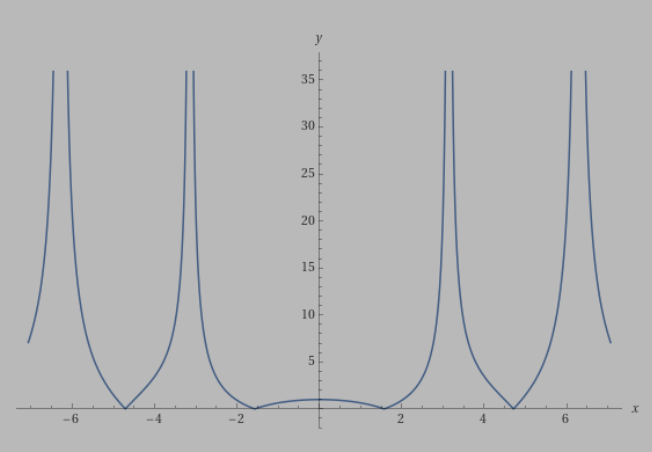
\includegraphics[width=0.5\linewidth]{image.png}
    \caption{Wykres funkcji $f(x) = |xcot(x)|$}
    \label{fig:enter-label}
\end{figure}

\begin{quote}
d) Problem jest czuły w miejscach, gdzie funkcja $\cot x$ zmierza do nieskończoności. Najlepiej uwarunkowany natomiast będzie w miejscach, gdzie funkcja $\cot x$ osiąga swoje minima.

Wniosek: Funkcja sinus jest najgorzej uwarunkowana w swoich miejscach zerowych i najlepiej w miejscach, gdzie przyjmuje wartość równą 1.
\end{quote}
\setlength{\parskip}{1em}
\begin{enumerate}
  \setcounter{enumi}{2}
  \item Błąd progresywny to wartość bezwględna z różnicy wartości rzeczywistej i przybliżonej. 
  Błąd wsteczny to wartość bezwzględna z różnicy argumentu wstawionego do funkcji i argumentu, dla którego przybliżona wartość funkcji jest wartością rzeczywistą.
\end{enumerate}

Rozpatrujemy funkcję w postaci:

$$
y=\sin x
$$

a) $\hat{y}=x, \hat{x}=\arcsin \hat{y}$

\begin{quote}
  Błąd progresywny: $\begin{aligned} |y-\hat{y}| &= |\sin x-x| \end{aligned}$ \\[1em]
  Błąd wsteczny: $\begin{aligned} |\hat{x}-x| &= |\arcsin \hat{y}-x| &= |\arcsin x-x| \end{aligned}$
  \end{quote}


b) $\hat{y}=x-\frac{x^{3}}{6}, \hat{x}=\arcsin \left(x-\frac{x^{3}}{6}\right)$

  \begin{quote}
  Błąd progresywny: $|y-\hat{y}|=\left|\sin x-\left(x-\frac{x^{3}}{6}\right)\right|=\left|\sin x+\frac{x^{3}}{6}-x\right|$
  
  Błąd wsteczny: $|\hat{x}-x|=|\arcsin \hat{y}-x|=\left|\arcsin \left(x-\frac{x^{3}}{6}\right)-x\right|$
  \end{quote}


Obliczenia do podpunktu a):
\begin{itemize}
  \item $x=0.1$ :
\end{itemize}

\begin{quote}
        $\hat{y}=x=0.1$

        $\hat{x}=\arcsin \hat{y} \approx 0.100167421$

        Błąd progresywny: $|\sin 0.1-0.1| \approx 0.000166583$

        Błąd wsteczny: $|\hat{x}-0.1| \approx 0.000167421$
  \end{quote}

\begin{itemize}
  \item $x=0.5$ :
\end{itemize}

\begin{quote}
        $\hat{y}=x=0.5$

        $\hat{x}=\arcsin \hat{y} \approx 0.523598776$

        Błąd progresywny: $|\sin 0.5-0.5| \approx 0.020574461$

        Błąd wsteczny: $|\hat{x}-0.5| \approx 0.023598776$
\end{quote}

\vspace{2cm}
\begin{itemize}
  \item $x=1.0$ :
\end{itemize}

\begin{quote}
        $\hat{y}=x=1.0$

        $\hat{x}=\arcsin \hat{y} \approx 1.570796327$

        Błąd progresywny: $|\sin 1.0-1.0| \approx 0,158529015$

        Bład wsteczny: $|\hat{x}-1.0| \approx 0.570796327$
\end{quote}

Obliczenia do podpunktu b):
\begin{itemize}
  \item $x=0.1$ :
\end{itemize}

\begin{quote}
$\hat{y}=0.1-\frac{(0.1)^{3}}{6} \approx 0.099833333$

$\hat{x}=\arcsin \hat{y} \approx 0.099999916 $

Błąd progresywny: $|\sin 0.1 + \frac{(0.1)^{3}}{6} -0.1| \approx 0.000000083$

Błąd wsteczny: $|\hat{x}-0.1| \approx 0.000000084$
\end{quote}
\begin{itemize}
  \item $x=0.5$ :
\end{itemize}

\begin{quote}
$\hat{y}=0.5-\frac{(0.5)^{3}}{6} \approx 0.479166666$

$\hat{x}=\arcsin \hat{y} \approx 0.499705041$

Błąd progresywny: $\left|\sin 0.5+\frac{(0.5)^{3}}{6}-0.5\right| \approx 0.000258872$

Błąd wsteczny: $|\hat{x}-0.5| \approx 0.000294959$
\end{quote}
\begin{itemize}
  \item $x=1.0$ :
\end{itemize}

\begin{quote}
$\hat{y}=1.0-\frac{(1.0)^{3}}{6} \approx 0.833333333$

$\hat{x}=\arcsin \hat{y} \approx 0.985110783$

Błąd progresywny: $\left|\sin 1 + \frac{(1.0)^{3}}{6}- 1 \right| \approx 0.008137652$

Błąd wsteczny: $|\hat{x}-1.0| \approx 0.014889216$
\end{quote}

Wniosek: Zwiększenie liczby wyrazów szeregu użytych do obliczeń skutkuje zwiększeniem ich dokładności.

\vspace{4cm}
4.

a) Poziom UFL to najmniejsza liczba dodatnia, którą możemy zapisać w danym systemie. Jest ona dana wzorem:

$$
U F L=\beta^{L}=10^{-98}
$$

b) $x-y=0.06 \times 10^{-97}=6 \times 10^{-99}<U F L$, stąd   $x-y$ = 0 w zadanym systemie.

Wniosek: Jeśli zamierzamy używać systemu do obliczania wartości operacj na bardzo małych liczbach to powinniśmy możliwie zminimalizować wartość $L$.

\end{document}
